% !TeX spellcheck = en_US
\documentclass[12pt, a4paper]{article}
\usepackage[scaled]{helvet}
\renewcommand\familydefault{\sfdefault}
\usepackage[T1]{fontenc}
\usepackage[margin=0.5in]{geometry}
\usepackage{float}
\usepackage{framed}
\usepackage{multicol}
\usepackage{amsmath}
\usepackage[framemethod=TikZ]{mdframed}
\usepackage{graphicx}
\usepackage{enumitem}
\setlist{nosep}
\usepackage{booktabs}
\usepackage{tikzsymbols}

\newcounter{note}\setcounter{note}{0}
\renewcommand{\thenote}{\arabic{note}}
\newenvironment{note}[1]{
	\stepcounter{note}
	\ifstrempty{#1}{
		\mdfsetup{
			frametitle={
				\tikz[baseline=(current bounding box.east),outer sep=0pt]
				\node[anchor=east,rectangle,fill=blue!20]
				{\strut Note~\thenote};
			}
		}
	}{
		\mdfsetup{
			frametitle={
				\tikz[baseline=(current bounding box.east),outer sep=0pt]
				\node[anchor=east,rectangle,fill=blue!20]
				{\strut Note~\thenote:~#1};
			}
		}
	}
	\mdfsetup{innertopmargin=0pt,linecolor=blue!20,linewidth=2pt,topline=true,frametitleaboveskip=\dimexpr-\ht\strutbox\relax}
	\begin{mdframed}[]\relax
}{
	\end{mdframed}
}

\begin{document}
	\tableofcontents
	\vspace{2em}
	\textbf{Contributors:}
	\begin{itemize}
		\item Daniel Fitz (Sanchez)
	\end{itemize}
	
	\section{Sem Outline}
	\begin{table}[H]
		\begin{tabular}{ll}
			Week (dates) & Lecture\\
			1 & Computer Networks and the Internet\\
			2 & Principles of Nw Apps: HTTP, SMTP, DNS\\
			3 & Application Layer: P2P, CDN, Sockets\\
			4 & Networking at UQ\\
			5 & Transport Layer: UDP\\
			6 & Transport Layer: TCP\\
			7 & Network Layer: Data Plane\\
			8 & Network Layer: Control Place\\
			9 & Link Layer\\
			11 & Wireless and Mobile\\
			12 & Security\\
			13 & Multimedia
		\end{tabular}
		\centering
		\caption{Week Outline}
	\end{table}


\newpage
\begin{multicols*}{2}
	
	\section{Exam Notes}
	The exam will consist of:
	\begin{itemize}
		\item A number of analytical questions, similar to the tutorial questions. You won't be asked any complex analytic problems which are completely different to those in tutorials
		\item A number of short answer questions of the type: compare XXX to YYY and explain the differences, or advantages/disadvantages of these protocols/algorithms/applications/techniques
		\item Questions about different protocols, their functions and where they fit in the network protocol stack. You won't be asked about protocols you have not seen in lectures
		\item Questions about packet exchanges in some common protocols (e.g. DHCP, DNS, ARP, TCP, HTTP)
	\end{itemize}
	\textit{No multiple choice questions this year \Sadey[][yellow!70] }
	\subsection{Chapter 1}
	\begin{itemize}
		\item What is the Internet
		\item Network Edge
		\item Network Core
		\item Delay, Loss Throughput
		\item Protocol Layers and their service models
	\end{itemize}
	\textit{Not Examinable:} Networks under attack, history of networking
	\subsection{Chapter 2: Application Layer}
	\begin{itemize}
		\item Principles of Networked Applications
		\item Web and HTTP (including options covered in lectures/labs)
		\item Electronic Mail
		\item DNS (but no detailed message/packet format)
		\item Peer-to-peer
		\item Internet Video
	\end{itemize}
	\textit{Not Examinable:} Detailed message formats for DNS and for email, case studies, socket programming
	\subsection{Chapter 3: Transport Layer}
	All Material
	\subsection{Chapter 4: Network Layer -- Data Plane}
	All Material
	\subsection{Chapter 5: Network Layer -- Control Plane}
	Most of the material covered, except as below, including a general overview of what SNMP does. You should understand link-state and distance vector routing. You won't be asked any numerical questions with distance-vector. For routing protocols, you should know about BGP, OSPF, IS-IS, RIP (which isn't in lectures, but is an example of an intra-AS distance-vector algorithm). All you really need to know about these algorithms are whether they are inter-AS or intra-AS, link-state or distance-vector.\\
	\textit{Not Examinable:} Details of SNMP architecture and packet formats. Details of BGP (5.4.2, 5.4.3, 5.4.5 are not examinable)
	\subsection{Chapter 6: Link Layer}
	\begin{itemize}
		\item General Principles
		\item Error Detection and Correction -- services provided, differences between correction and detection
		\item Multiple Access Links and Protocols, but NOT DOCSIS
		\item Switched Local Area Networks
		\item ``Day in the Life of a Web Page Request'' -- details of each stage are covered in the earlier sections
	\end{itemize}
	\textit{Not Examinable:} Exactly how to calculate parity, checksum, CRC, DOCSIS, MPLS, Data Center Networking
	\subsection{Chapter 7: Wireless}
	\begin{itemize}
		\item General Principles
		\item Wireless characteristics
		\item WiFi (IEEE 802.11) except as below
	\end{itemize}
	\textit{Not Examinable:} Mobility in WiFi, advanced features in WiFi (Ch 7.3.5). Personal area Networks. Cellular Internet Access. Mobility Management, Mobile IP, Mobility effects on higher layers
	\subsection{Chapter 8: Security}
	\begin{itemize}
		\item What is network security -- confidentiality, integrity, authentication
		\item Cryptographic principles -- symmetric and public key algorithms (you won't be asked to calculate any ciphers)
		\item Names, types and uses of common cyphers, at least: Diffie-Hellman, RSA, DES, 3DES, AES, MD5, SHA-1
		\item Message integrity and signatures
		\item SSL and TLS
		\item IP Sec and VPN
		\item Firewalls and Intrusion Detection Systems -- general principles
	\end{itemize}
	\textit{Not Examinable:} Details of cipher algorithms, key lengths. Securing Email. Wireless security
	\subsection{Chapter 9: Multimedia}
	\begin{itemize}
		\item Properties of multimedia
		\item UDP and HTTP streaming
		\item Voice over IP
		\item Protocols -- RTP, SIP
	\end{itemize}
	\textit{Not Examinable:} Case Studies (e.g. Skype). Network Support for multimedia, such as token-bucket, diffserv, QoS
	\subsection{Packet Formats}
	Must understand and decode the packet contents if given a byte stream for:
	\begin{description}
		\item[Link Layer:] Ethernet (but not VLAN packets)
		\item[Network Layer:] IPv4 (not IPv6), you won't be asked to decode option fields, but they may be present. These IPv4 packets may contain protocols like DNS or ICMP, but you won't be asked to decode the contents of those packets
		\item[Transport Layer:] TCP, UDP.. You won't be asked to decode option fields, by they may be present
		\item[Application Layer:] Simple HTTP request and reply. If you are required to decode text messages you will be given a table of ASCII codes
	\end{description}
	\newpage
	
	\section{Chapter 1}
	% !TeX spellcheck = en_US
% !TeX root = notes.tex
\begin{itemize}
	\item billions of connected computing devices
	\item transmission rate: \textbf{bandwidth}
	\item \textbf{Packet Switches:} Forward packets
	\begin{itemize}
		\item \textbf{routers} and \textbf{switches}
	\end{itemize}
	\item \textbf{Internet: ``network of networks''} (Interconnected ISPs)
	\item \textbf{Protocols} control sending, receiving (e.g. TCP, IP, HTTP, Skype, 802.11)
	\item \textbf{Internet standards}
	\begin{description}
		\item[RFC:] Request for comments
		\item[IETF:] Internet Engineering Task Force
	\end{description}
\end{itemize}

\subsection{Network Structure}
\begin{itemize}
	\item \textbf{Network Edge}
	\begin{itemize}
		\item hosts: clients and servers
		\item servers often in data centers
	\end{itemize}
	\item \textbf{Access networks, physical media:} wired, wireless communication links
	\item \textbf{network core:}
	\begin{itemize}
		\item interconnected routers
		\item network of networks
	\end{itemize}
\end{itemize}

\subsection{Access Network}
\subsubsection{Digital Subscriber Line (DSL)}
\begin{itemize}
	\item use \textbf{existing} telephone line to central office DSLAM
	\begin{itemize}
		\item data over DSL phone line goes to Internet
		\item voice over DSL phone line goes to telephone net
	\end{itemize}
	\item < 2.5 Mbps upstream transmission rate (typically < 1 Mbps)
	\item < 24 Mbps downstream transmission rate (typically < 10 Mbps)
\end{itemize}
\subsubsection{Cable Network}
\begin{leftbar}
	\textbf{frequency division multiplexing:} different channels transmitted in different frequency bands
\end{leftbar}
\begin{itemize}
	\item \textbf{HFC: hybrid fiber coax}
	\begin{itemize}
		\item asymmetric: up to 30Mbps downstream transmission rate, 2 Mbps upstream transmission rate
	\end{itemize}
	\item \textbf{network} of cable, fiber attaches homes to ISP router
	\begin{itemize}
		\item homes \textbf{share access network} to cable head-end
		\item unlike DSL, which has dedicated access to central office
	\end{itemize}
\end{itemize}
\textbf{wireless LANS:}
\begin{itemize}
	\item within building (30 meters)
	\item 802.11b/g/n (WiFi): 11,54,450 Mbps transmission rate
\end{itemize}
\textbf{wide-area wireless access:}
\begin{itemize}
	\item provided by telco (cellular) operator, 10's km
	\item between 1 and 10 Mbps
	\item 3G, 4G, LTE
\end{itemize}

\subsection{Sending}
\begin{itemize}
	\item takes application message
	\item breaks into smaller chunks, known as \textbf{packets}, of length \textbf{$L$} bits
	\item transmites packet into access network at \textbf{transmission rate $R$}
	\begin{itemize}
		\item link transmission rate, aka link \textbf{capacity, aka link bandwidth}
	\end{itemize}
\end{itemize}
\begin{note}{Packet Transmission Delay}
	\[
		\text{\parbox{2cm}{packet transmission delay}}=\text{\parbox{2cm}{time needed to transmit $L$-bit packet into link}}=\frac{L\text{ (bits)}}{R\text{ (bits/sec)}}
	\]
\end{note}

\subsection{Physical Media}
\begin{itemize}
	\item \textbf{bit:} propagates between transmitter/receiver pairs
	\item \textbf{physical link:} what lies between transmitter and receiver
	\item \textbf{guided media:} signals propagate in solid media (copper, fiber, coax)
	\item \textbf{unguided media:} signals propagate freely, e.g. radio
	\item \textbf{twisted pair (TP):} two insulated copper wires
	\begin{itemize}
		\item Category 5: 100 Mbps, 1 Gbps Ethernet
		\item Category 6: 10 Gbps
	\end{itemize}
\end{itemize}
\subsubsection{Coax}
\begin{itemize}
	\item two concentric copper conductors
	\item bidirectional
	\item broadband: multiple channels on cable, HFC
\end{itemize}
\subsubsection{Fiber Optic Cable}
\begin{itemize}
	\item glass fiber carrying light pulses, each pulse a bit
	\item high-speed operation: high-speed point-to-point transmission (e.g. 10's - 100's Gbps transmission rate)
	\item low error rate
	\begin{itemize}
		\item repeaters spaced far apart
		\item immune to electromagnetic noise
	\end{itemize}
\end{itemize}
\subsubsection{Radio}
\begin{itemize}
	\item signal carried in electromagnetic spectrum
	\item no physical "wire"
	\item bidirectional
	\item propagation environment effects:
	\begin{itemize}
		\item reflection
		\item obstruction by objects
		\item interference
	\end{itemize}
\end{itemize}
\textbf{Radio Link Types:}
\begin{itemize}
	\item \textbf{terrestrial microwave:} up to 45 Mbps channels
	\item \textbf{LAN} (e.g. WiFi) 54 Mbps
	\item \textbf{wide-area} (e.g. cellular) 4G cellular: \~ 10 Mbps
	\item \textbf{satellite}
	\begin{itemize}
		\item Kbps to 45 Mbps channel (or multiple smaller channels)
		\item 270 msec end-end delay
		\item geosynchronous versus low altitude
	\end{itemize}
\end{itemize}

\subsection{Packet-switching}
\subsubsection{Store-and-forward}
\begin{leftbar}
	$L$ bits per packet\\
	Source to destination: $R$ bps
\end{leftbar}
\begin{itemize}
	\item takes $\frac{L}{R}$ seconds to transmit (push out) $L$-bit packet into link at $R$ bps
	\item \textbf{store and forward:} entire packet must arrive at router before it can be transmitted on next link
\end{itemize}
\begin{note}{End-End delay}
	\[
		\text{delay} = 2\frac{L}{R}
	\]
	(assuming zero propagation delay)
\end{note}
\subsubsection{Packet switching versus circuit switching}
Is packet switching a ``slam dunk winner?''
\begin{itemize}
	\item great for bursty data (resource sharing, simpler, no call setup)
	\item excessive congestion possible: packet delay and loss (protocols needed for reliable data transfer, congestion control)
\end{itemize}

\subsection{Packet Loss}
\begin{figure}[H]
	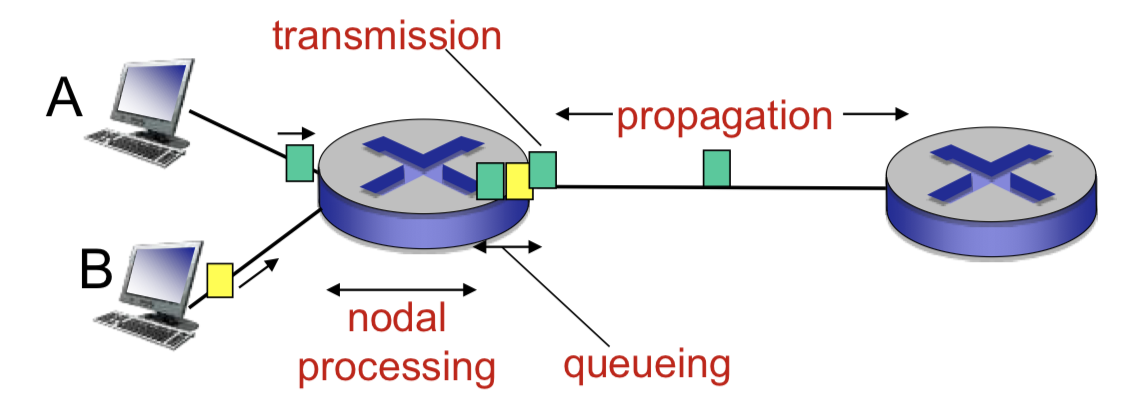
\includegraphics[width=8cm]{delay}
	\centering
	\caption{Packet Delay Algorithm Explanation}
\end{figure}
\begin{note}{Packet Delay Algorithm}
	\[ d_\text{nodal} = d_\text{proc} + d_\text{queue} + d_\text{trans} + d_\text{prop} \]
\end{note}
\subsubsection{Nodal Processing}
\[ d_\text{proc} \]
\begin{itemize}
	\item check bit errors
	\item determine output link
	\item typically < msec
\end{itemize}
\subsubsection{Queuing Delay}
\[ d_\text{queue} \]
\begin{itemize}
	\item time waiting at output link for transmission
	\item depends on congestion level of router
\end{itemize}
\subsubsection{Transmission Delay}
\[ d_\text{trans} \]
\begin{itemize}
	\item $L$: packet length (bits)
	\item $R$: link bandwidth(bps)
	\item $d_\text{trans} = \frac{L}{R}$
\end{itemize}
\subsubsection{Propagation Delay}
\[ d_\text{prop} \]
\begin{itemize}
	\item $d$: length of physical link
	\item $s$: propagation speed ($\approx2\times10^8$ m/sec)
	\item $d_\text{prop} = \frac{d}{s}$
\end{itemize}

\subsection{Throughput}
\begin{leftbar}
	Rate (bits/time unit) at which bits transferred between sender/receiver
\end{leftbar}
\begin{description}
	\item[Instantaneous:] rate at given point in time
	\item[Average:] rate over longer period of time
\end{description}
\begin{note}{Bottleneck Link}
	Link on end-end path that constrains end-end throughput
\end{note}

\subsection{Layering}
\subsubsection{Why Layering?}
Dealing with complex systems:
\begin{itemize}
	\item Explicit structure allows identification, relationship of complex system's pieces (layered \textbf{reference model} for discussion)
	\item Modularization eases maintenance, updating system
	\begin{itemize}
		\item change of implementation of layer's service transparent to rest of system
		\item e.g. change in gate procedure doesn't affect rest of system
	\end{itemize}
	\item layering considered harmful?
\end{itemize}
\subsubsection{Internet Protocol Stack}
\begin{description}
	\item[Application:] supporting network applications (FTP, SMTP, HTTP)
	\item[Transport:] process-process data transfer (TCP, UDP)
	\item[Network:] routing of datagrams from source to destination (IP, routing protocols)
	\item[Link:] data transfer between neighboring network elements (Ethernet, 802.111 (WiFi), PPP)
	\item[Physical:] bits ``on the wire''
\end{description}
\subsubsection{ISO/OSI Reference Model}
Internet stack ``missing'' these layers. These services, if needed, must be implemented in application.
\begin{description}
	\item[Application:]
	\item[Presentation:] allow applications to interpret meaning of data, e.g. encryption, compression, machine-specific conventions
	\item[Session:] synchronization, check-pointing, recovery of data exchange
	\item[Transport:]
	\item[Network:]
	\item[Link:]
	\item[Physical:]
\end{description}

\subsection{Security}
\begin{itemize}
	\item Malware can get in host from:
	\begin{description}
		\item[Virus:] self-replicating infection by receiving/executing object (e.g. e-mail attachment)
		\item[Worm:] self-replicating infection by passively receiving object that gets itself executed
	\end{description}
	\item \textbf{Spyware malware} can record keystrokes, web sites visited, upload info to collection site
	\item Infected host can be enrolled in \textbf{botnet}, used for spam. DDoS attacks
\end{itemize}
\subsubsection{DoS: Denial of Service}
\textbf{Denial of Service (DoS):} attackers make resources (server, bandwidth) unavailable to legitimate traffic by overwhelming resource with bogus traffic
\begin{enumerate}
	\item select target
	\item break into hosts around the network (botnet)
	\item send packets to target from compromised hosts
\end{enumerate}
\subsubsection{Sniffing}
\begin{itemize}
	\item broadcast media (shared Ethernet, wireless)
	\item promiscuous network interface reads/records all packets (e.g. including passwords) passing by
\end{itemize}
\subsubsection{IP Spoofing}
Send packet with false source address
	
	\section{Chapter 2}
	% !TeX spellcheck = en_US
% !TeX root = notes.tex
\subsection{Application Architectures}
\subsubsection{Client-Server}
\begin{description}
	\item[Server:] Always-on host, Permanent IP address
	\item[Clients:] Do not communicate directly with each other, May have dynamic IP addresses
\end{description}

\subsubsection{Peer-to-Peer (P2P)}
\begin{itemize}
	\item No always-on server
	\item Peers request service from other peers, provide service in return to other peers
	\item \textbf{Self Scalability} -- new peers bring new service capacity, as well as new service demands
	\item Pers are intermittently connected and change IP addresses
\end{itemize}

\begin{note}{App-layer protocol defines}
	\begin{itemize}
		\item \textbf{type of messages exchanged} -- e.g. request, response
		\item \textbf{message syntax} -- what fields in messages and how fields are delineated
		\item \textbf{message semantics} -- meaning of information in fields
		\item \textbf{rules} for when and how processes send and respond to messages
		\item \textbf{open protocols} -- defined in RFCs, allows for interoperability (e.g. HTTP, SMTP)
		\item \textbf{proprietary protocols} -- e.g. Skype
	\end{itemize}
\end{note}

\subsection{Transport Service is needed}
\begin{description}
	\item[Data Integrity:] Some programs need 100\% reliable data transfer (e.g. file transfer, web transactions), others can tolerate loss (e.g. audio)
	\item[Timing:] Some programs require low delay to be ``effective'' (e.g. online games)
	\item[Throughput:] Some programs require minimum amount of throughput to be ``effective'' (e.g. multimedia), some use whatever they have available (``elastic apps'')
	\item[Security:] Encryption, Data Integrity
\end{description}

\subsection{Transport Protocol Services}
\subsubsection{TCP}\label{sec:tcp}
\begin{description}
	\item[Reliable Transport] between sending and receiving process
	\item[Flow Control:] sender won't overwhelm receiver
	\item[Congestion Control:] throttle sender when network overloaded
	\item[Connection-Oriented:] setup required between client and server processes
	\item[Does Not Provide:] timing, minimum throughput guarantee, security
\end{description}

\subsubsection{UDP}\label{sec:udp}
\begin{description}
	\item[Unreliable Data Transfer] between sending and receiving process
	\item[Does Not Provide:] reliability, flow control, congestion control, timing, throughput guarantee, security, or connection setup
\end{description}

\subsubsection{Securing TCP}
\textbf{TCP and UDP}
\begin{itemize}
	\item no encryption
	\item cleartext passwords sent into socket traverse Internet in cleartext
\end{itemize}
\textbf{SSL}
\begin{itemize}
	\item provides encrypted TCP connection
	\item data integrity
	\item end-point authentication
\end{itemize}
\textbf{SSL is at app layer}
\begin{itemize}
	\item app use SSL libraries, that ``talk'' to TCP
\end{itemize}
\textbf{SSL socket API}
\begin{itemize}
	\item cleartext passwords sent into socket traverse Internet encrypted
\end{itemize}

\subsection{HTTP: Hypertext Transfer Protocol}\label{sec:http}
\begin{itemize}
	\item Web's application layer protocol
	\item client/server model. Client request website and server serves HTTP object in response
	\item Uses TCP
	\item HTTP is stateless. Server maintains no information about past client requests
	\item \textbf{non-persistent HTTP:} one object sent over one TCP connection, downloading multiple object required multiple connections
	\item \textbf{persistent HTTP:} multiple object sent over single TCP connection
\end{itemize}
Non-persistent HTTP issues:
\begin{itemize}
	\item requires 2 RTTs per object
	\item OS overhead for each TCP connection
	\item browsers often open parallel TCP connections to fetch referenced objects
\end{itemize}
Persistent HTTP:
\begin{itemize}
	\item server leaves connection open after sending response
	\item subsequent HTTP messages between same client/server sent over open connection
	\item client sends requests as soon as it encounters a referenced object
	\item as little as one RTT for all the referenced objects
\end{itemize}
\subsubsection{Method Types}
\textbf{HTTP/1.0:} GET, POST, HEAD (asks server to leave requested object out of response)\\
\textbf{HTTP/1.1:} GET, POST, HEAD, PUT (uploads file in entity body to path specified in URL field), DELETE (deletes file specified in the URL field)
\subsubsection{Response Codes}
\begin{description}
	\item[200 OK:] request succeeded, requested object later in this msg
	\item[301 Moved Permanently:] requested object moved, new location specified later in this msg
	\item[400 Bad Request:] request msg not understood by server
	\item[404 Not Found:] requested document not found on this server
	\item[505 HTTP Version Not Supported]
\end{description}

\subsection{Cookies}
Uses: authorization, shopping carts, recommendations, user session state (Web, email)

\subsection{Web Caches (proxy server)}
\begin{leftbar}
	\textbf{Goal:} satify client request without involving origin server
\end{leftbar}
\begin{itemize}
	\item Browsers requests object from cache, if in cache the object is sent back otherwise cache requests object from origin
	\item Cache acts as both client and server
	\item Reduce response time for client request
	\item Reduce traffic
\end{itemize}

\subsubsection{Conditional GET}
\begin{leftbar}
	\textbf{Goal:} don't send object if cache has up-to-date cached version (lower link usage)
\end{leftbar}
\begin{itemize}
	\item \textbf{Cache:} specify date of cached copy in HTTP request \texttt{If-modified-since: <date>}
	\item \textbf{Server:} response contains no object if cached copy is up-to-date: \texttt{HTTP/1.0 Not Modified}
\end{itemize}

\subsection{Electronic Mail: SMTP}\label{sec:smtp}
\textit{RFC 2821}
\begin{itemize}
	\item uses TCP to reliably transfer email message from client to server, port 25
	\item direct transfer: sending server to receiving server
	\item three phases of transfer: handshaking, transfer of messages, closure
	\item command/response interaction
	\item messages must be in 7-bit ASCII
	\item uses persistent connections
	\item requires message to be in 7-bit ASCII
	\item uses \texttt{CRLF.CRLF} to determine end of message
\end{itemize}
Difference to HTTP being, HTTP is server sending data, SMTP is client connection sending data\\
\begin{description}
	\item[SMTP:] protocol for exchanging email messages
	\item[RFC 822:] standard for text message format (To, From, Subject, Body)
\end{description}
\subsubsection{Mail Access Protocols}
\begin{leftbar}
	\textbf{SMTP:} delivery/storage to receiver's server
\end{leftbar}
\begin{description}
	\item[POP:] Post Office Protocol \textit{(RFC 1939)}: authorization, download
	\begin{itemize}
		\item POP3 is stateless across sessions
		\item Two main modes; download and delete, download and keep (allows multiple clients to read the same email)
	\end{itemize}
	\item[IMAP:] Internet Mail Access Protocol \textit{(RFC 1730)}: more features, including manipulation of stored message on server
	\begin{itemize}
		\item All messages stored on server
		\item Supports folders
		\item Keeps user state across sessions: names of folders and mappings between message IDs and folder name
	\end{itemize}
	\item[HTTP:] gmail, Hotmail, Yahoo, etc
\end{description}

\subsection{DNS: Domain Name System}\label{sec:dns}
\begin{itemize}
	\item Lookup between names (e.g. google.com) and IP addresses
	\item \textbf{Distributed Database} implemented in hierarchy of many \textbf{name servers}
	\item \textbf{Application-layer protocol:} hosts, name servers communicate to \textbf{resolve} names (address/name translation)
\end{itemize}
Why not centralize DNS? Single point of failure, traffic volume, doesn't scale
\subsubsection{DNS Services}
\begin{itemize}
	\item hostname to IP address translation
	\item host aliasing (canonical, alias names)
	\item mail server aliasing
	\item load distribution (many IP addresses correspond to one name)
\end{itemize}
\subsubsection{TLD, authoritative servers}
\textbf{top-level domain (TLD) servers:}
\begin{itemize}
	\item responsible for com, org, net, edu, aero, jos, io
	\item and top-level country domains au, uk, ca
	\item Network Solutions maintains servers for .com TLD
	\item Educause for .edu TLD
\end{itemize}
\textbf{Authoritative DNS servers:}
\begin{itemize}
	\item organization's own DNS server(s), providing authorative hostname to IP mappings for organization's named hosts
	\item can be maintained by organization or service provider
\end{itemize}
\subsubsection{Local DNS name server}
\begin{itemize}
	\item does not strictly belong to hierarchy
	\item each ISP (residential ISP, company, university) has one (also called ``default name server'')
	\item when host makes DNS query, query is sent to its local DNS server
	\begin{itemize}
		\item has local cache of recent name-to-address translation pairs (but may be out of date!)
		\item acts as proxy, forwards query into hierarchy
	\end{itemize}
\end{itemize}
\subsubsection{DNS Name Resolution}
\begin{description}
	\item[Iterated query:] contacted server replies with name of server to contact. So root dns sends the ip of the next dns server to contact
	\item[Recursive query:] puts burden of name resolution on contacted name server. So root dns server contacts the next levels down which contacts next level down.
\end{description}
\subsubsection{Caching}
Once (any) name server learns mapping, it \textbf{caches} mapping. Cache entries timeout (disappear) after some time (TTL). If name host changes IP address, the name servers might not update until TTLs expire.
\begin{leftbar}
	update/notify mechanisms proposed IETF standard RFC 2136
\end{leftbar}
\subsubsection{DNS Records}
\begin{note}{RR Format}
	\texttt{(name, value, type, ttl)}
\end{note}
\begin{description}
	\item[type=A] \texttt{name} is hostname, \texttt{value} is IP address
	\item[type=NS] \texttt{name} is domain (e.g. google.com), \texttt{value} is hostname of authoritative name server for this domain
	\item[type=CNAME] \texttt{name} is alias name for some ``canonical'' (the real) name (\texttt{www.ibm.com} is really \texttt{servereast.backup2.ibm.com}), \texttt{value} is canonical name
	\item[type=MX] \texttt{value} is name of mailserver associated with \texttt{name}
\end{description}
\subsubsection{Protocol}
Query and reply messages both follow same format
\begin{table}[H]
\centering
\caption{Protocol Layout}
\begin{tabular}{cc}
	\toprule
	2 bytes & 2 bytes \\
	\midrule
	identification & flags\\
	\# questions & \# answer RRs\\
	\# authority RRs & \# additional RRs\\
	\multicolumn{2}{c}{questions (variable \# of questions)}\\
	\multicolumn{2}{c}{answers (variable \# of RRs)}\\
	\multicolumn{2}{c}{authority (variable \# of RRs)}\\
	\multicolumn{2}{c}{additional info (variable \# of RRs)}\\
	\bottomrule
\end{tabular}
\end{table}
\subsubsection{Attacking DNS}
\textbf{DDoS attacks}
\begin{itemize}
	\item bombard root servers with traffic. Not successful to date, traffic filtering, local DNS servers cache protecting root DNS
	\item bombard TLD server. Potentially more dangerous
\end{itemize}
\textbf{Redirect Attacks}
\begin{itemize}
	\item man-in-middle (Intercept queries)
	\item DNS Poisoning (Send bogus relies to DNS server, which caches)
\end{itemize}
\textbf{Exploit DNS for DDoS}
\begin{itemize}
	\item send queries with spoofed source address: target IP
	\item requires amplification
\end{itemize}
	% !TeX spellcheck = en_US
% !TeX root = notes.tex
\section{Lecture 3: Bitcoin, Cryptocurrencies Blockchain Technology}
\subsection{Sybil Attack}
\begin{itemize}
	\item The Sybil attack in computer security is an attack wherein a reputation system is subverted by forging identities in peer-to-peer networks.
	\item Creates a large number of false identities in order to flood the network and take it over.
	\item Named after the subject of the book \textbf{Sybil}, a case study of a woman diagnosed with multiple personality disorder
	\item Such false identities are called \textbf{``Sybils''}, in the context of P2P systems
	\item One approach to preventing these “Sybil attacks” is to have a trusted agency certify identities.
	\item Or \textbf{``Sockpuppets''} in the context of the Internet, e.g. to manipulate public opinion
	\begin{leftbar}
		``... referred to a false identity assumed by a member of an Internet community who spoke to, or about, themselves while pretending to be another person. `The term now includes other misleading uses of online identities, such as those created to praise, defend or support a person or organization, to manipulate public opinion, or to circumvent a suspension or ban from a website''\\
		- Wikipedia
	\end{leftbar}
\end{itemize}

\subsection{Decentralized Consensus in Bitcoin}
\begin{itemize}
	\item Bitcoin achieves consensus by replacing \textbf{one node (or one IP address) one vote}, with \textbf{one CPU one vote}
	\item Bitcoin mining uses mostly ASICs and GPUs, not CPUs
	\item Consensus is achieved by a (probabilistic) majority vote, based on computing power
	\begin{itemize}
		\item Attacker needs > 50\% of combined computing power in order to cheat with high probability
		\item This is harder to achieve than controlling more than half of the nodes
		\item It's relatively easy to spin up a few thousand VMs as nodes, compared to controlling >50\% of Bitcoin's mining compute power
	\end{itemize}
	\item Bitcoin combines a \textbf{proof-of-work mechanism} (based on Hashcash), combined with a clever incentive mechanism $\rightarrow$ Nodes get paid to do the right thing, i.e. checking and confirming valid transactions via ``mining''
\end{itemize}

\section{Lecture 3: Bitcoin}
\begin{itemize}
	\item Complete transaction history is stored in public ledger (blockchain), stored by nodes in P2P network
	\item New transactions are created off-line, and then broadcast is P2P network
	\item Nodes validate and relay transactions (if valid)
	\item Nodes add new transactions (not part of blockchain yet) to a \textbf{transaction pool}
	\item Nodes combine transactions in pool to a block, and try to solve the corresponding proof-of-work puzzle, to ``confirm'' the block
	\item Node that finds solution first broadcasts block with solution in the network (Winning node selection is probabilistic, with probability propertional to computing power)
	\item Nodes check solution, and if OK, add new block to their local copy of blockchain
	\item All nodes who were working on solving the old puzzle, immediately start working on a new block
	\begin{itemize}
		\item Everybody always works on the longest chain
		\item Convergence to longest chain provides consensus
		\item Forks happen but are resolved by (computational) majority vote
	\end{itemize}
\end{itemize}
\begin{note}{Bitcoin Components}
	\begin{itemize}
		\item Bitcoin Network
		\item Bitcoin Identities/Addresses
		\item Bitcoin Transactions
		\item Bitcoin Scripting Language
		\item Blocks
		\item Proof-of-work, Hash puzzles, Mining
		\item Consensus
	\end{itemize}
\end{note}

\subsection{Bitcoin Network}
Transactions are broadcast in the Bitcoin network, consisting of ``full'' Bitcoin nodes ($\approx$10,000)
\begin{itemize}
	\item Best-effort (asynchronous, unreliable), it's enough if only some nodes get the message
	\item It's easy to join the Bitcoin Network, just download and run the client (Bitcoin is a \textbf{permissionless, public} blockchain, anyone can join)
\end{itemize}
Network is unstructured P2P network (random topology)
\begin{itemize}
	\item Similar to Gnutella (a P2P system from a long time ago)
	\item Overlay network, TCP, port 8333
	\item Messages are flooded
	\item All nodes are equal, no hierarchy
	\item Nodes can join at any time
	\item Node is `forgotten' if it does not respond for more than 3 hours
	\item Network is very simple and robust, e.g. to churn, but not very efficient
\end{itemize}
\begin{note}{Bitcoin Network Nodes}
	\begin{itemize}
		\item Check validity of transactions
		\item Relay transactions in the network via flooding
		\item Mining (proof-of-work puzzles)
		\item Validate and forward confirmed blocks (Add them to local copy of blockchain)
	\end{itemize}
\end{note}
\subsection{Bitcoin Identity and Addresses}
Users are represented by their Public Key addresses (hash), called \textbf{Bitcoin Addresses}, which serve as a pseudonyms
\begin{itemize}
	\item An address is a \textbf{160 bit} value, and is computed as follows
	\item RIPEMD160 hash of SHA-256 hash of ECDSA Public Key
	\item This is a ``Pay-to-pubkey-hash (P2PKH)'' address, encoding starts with ``1''
\end{itemize}
When spending a coin, spender needs to proof ownership of coin by providing a valid digital signature on the spend transaction (i.e. proving ownership of corresponding private key)\\
How can digital signatures be verified?
\begin{itemize}
	\item We need public key, not just hash of public key
	\item Spender of coin needs to provide both valid signature AND public key
	\item How do we know the provided public key is authentic $\rightarrow$ Hash it, and compare with Bitcoin address, which is the hash of public key
\end{itemize}
Bitcoin also supports \textbf{Pay to script hash (P2SH)} addresses
\begin{itemize}
	\item Allow transactions to be sent to a \textbf{script hash} instead of a public key hash (Address encoding starts with a `3' instead of `1')
	\item To spend bitcoins sent via P2SH, the recipient must provide a script matching the script hash and data which makes the script evaluate to true
	\item Allows more complex transactions (\textbf{smart contracts}), e.g. transaction outputs that require multiple signatures (multisig), or transaction puzzle, ...
\end{itemize}
\begin{note}{Bitcoin Address Encoding}
	Bitcoin uses Base58 encoding (binary-to-text encoding). Similar to Base64 encoding, but without some characters. Rationale, as explained in original bitcoin client source code:
	\begin{code}
		// Why base-58 instead of standard base-64 encoding?\\
		// - Don't want 0OIL characters that look like the same in some fonts and\\
		//   could be used to create visually identical looking account numbers.\\
		// - A string with non-alphanumeric characters is not as easily accepted as an account nbr.\\
		// - E-mail usually won't line-break if there's no punctuation to break at.\\
		// - Doubleclicking selects the whole number as one word if it's all\\alphanumeric.
	\end{code}
	Bitcoin also adds 4 byte checksum to addresses
\end{note}
\subsubsection{Bitcoin Address -- Balance}
\begin{itemize}
	\item The ``balance'' of an address is the total of unspent transaction outputs (UTXO) sent to the address.
	\item ``There are no accounts or balances in bitcoin; there are only unspent transaction outputs (UTXO) scattered in the blockchain''
	\item A user typically has many different addresses, all managed by the ``wallet'' software
	\item The wallet ``balance'' is the sum of all unspent transaction outputs of all addresses owned by the user
\end{itemize}
\subsection{Bitcoin Transactions}
\begin{itemize}
	\item Transaction are created off-line (No need to be connected to Bitcoin network for this)
	\item Transactions are broadcast in Bitcoin P2P network
	\item Nodes check validity, and relay transaction (flooding)
	\item Nodes add to new transactions to a block and try to solve hash puzzle
	\item A block with a solved puzzle is ``confirmed'', and broadcast in the network, and added to the blockchain of each node
	\item Contains:
	\begin{itemize}
		\item Inputs (any number $\geq0$)
		\item Outputs (any number > 0)
		\item Digital signatures of input coin owners (Typically for \textbf{P2PKH} transactions)
		\item Input needs to be completely consumed (With exception of Transaction Fee)
	\end{itemize}
\end{itemize}
\subsubsection{Basic Transaction Types}
\begin{itemize}
	\item Common Transaction
	\begin{itemize}
		\item 1 input
		\item 1 ``normal'' output
		\item 1 change output (back to owner)
		\subitem Create new ``Change Address'' to maintain ``anonymity''
	\end{itemize}
	\item Aggregating Transaction
	\begin{itemize}
		\item Multiple inputs
		\item 1 output
	\end{itemize}
	\item Distributing Transaction
	\begin{itemize}
		\item 1 input
		\item Multiple outputs
	\end{itemize}
	\item ``Coinbase Transaction''
	\begin{itemize}
		\item 0 input, 1 outputs
		\item Freshly created (``minted'') coins
		\item Miner gets this as a reward for solving Hash puzzle (and thereby confirming block)
		\item First transaction in every block
	\end{itemize}
\end{itemize}

\subsection{Bitcoin Scripts}
\begin{itemize}
	\item Two types of Bitcoin scripts to validate transactions
	\begin{itemize}
		\item a locking script (Typically \textbf{ScriptPubKey})
		\item and an unlocking script (Typically \textbf{ScriptSig})
	\end{itemize}
	\item A locking script is a condition placed on an output
	\item It specifies the conditions that must be met to spend or consume the output in the future
	\begin{itemize}
		\item Typically a \textbf{valid digital signature} of the claimed owner
		\item Can be other things, to implement basic `smart contracts'
	\end{itemize}
\end{itemize}
\subsubsection{Bitcoin Scripting Language ``Script''}
\begin{itemize}
	\item Allows to program conditions required for the spending of Bitcoins (``Programmable Money'')
	\item \textbf{Script} is a simple, stack based language
	\item Not Turing complete (e.g. no loops)
	\item Scripts are guaranteed to terminate after a fixed number of steps, e.g. no infinite loops
	\item Why is this a good thing?
	\begin{itemize}
		\item Avoids potential denial of service attacks on nodes, ``logic bombs''
		\item Remember: Every node runs all scripts to validate all transactions (BTW, this severely limits scalability of Bitcoin)
	\end{itemize}
	\item In contrast, Ethereum has a Turing complete scripting language
	\subitem Solves DoS attack problem by putting a price on script computation (`Gas')
\end{itemize}

\subsection{Blocks}
\begin{itemize}
	\item Transactions are grouped into blocks
	\subitem This is an optimization. Confirming individual transactions and adding them to the blockchain would be possible, but very inefficient
	\item Transactions are stored in a Merkle Tree, with the Merkle Root (Tx\_Root) stored in the block header
	\item Once confirmed (via solving hash puzzle), a block is added to the blockchain
	\item The `Nonce' is the solution of the hash puzzle
\end{itemize}
\begin{figure}[H]
	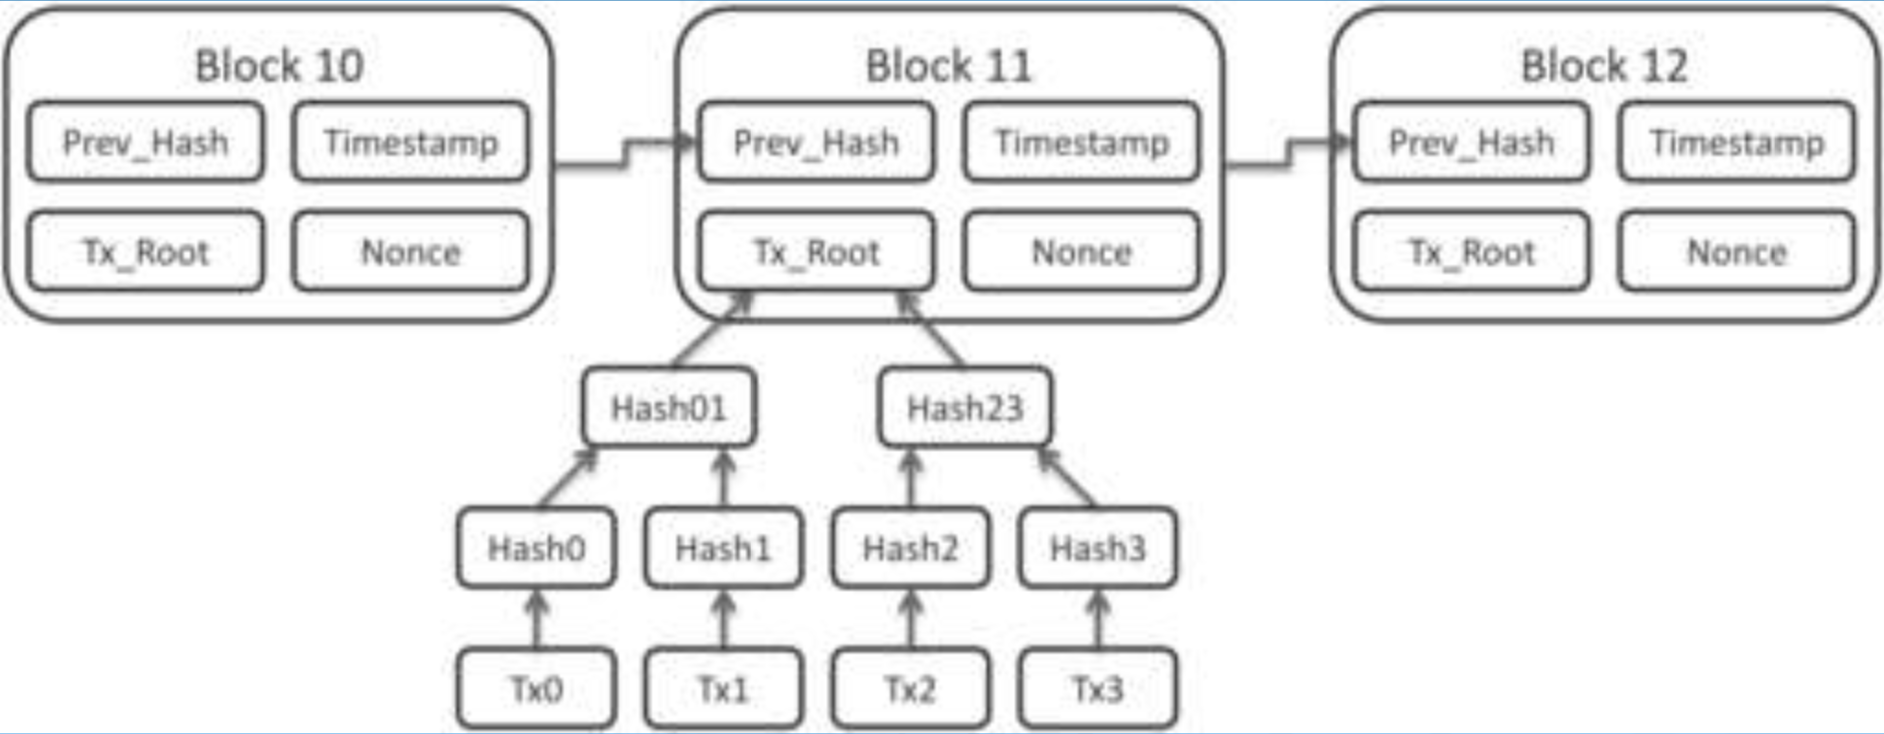
\includegraphics[width=\linewidth]{blockStructure}
	\centering
	\caption{Block Structure}
\end{figure}
\subsubsection{How are blocks added to the Blockchain?}
\begin{itemize}
	\item Multiple nodes (miners) are working towards solving the hash puzzle for a new block
	\subitem miners are probably working on different version of blocks, depending on content on their transaction pool
	\item First node who solves puzzle, broadcasts new block with solution (nonce) in the Bitcoin P2P network
	\begin{itemize}
		\item Choice of winning node is random (probabilistic)
		\item Probability of success is proportional to computing power of miner
	\end{itemize}
	\item ``Block Height'' is sequence number of blocks
	\item Other nodes check if solution is correct, and if so, add block to their local copy of the blockchain, and forward new block to other nodes
\end{itemize}

\subsection{Bitcoin Mining}
\begin{itemize}
	\item At the current level of difficulty, solving Bitcoin hash puzzles is hard and expensive
	\item Mostly ASICs based, some GPUs
	\item Total hash rate of entire Bitcoin network $\approx25\times10^{18}$H/s
	\item Hash rate of an Intel i7 CPU $\approx10$MH/s
	\subitem Need > 10,000,000 laptops to be able to mine one block per year on average
	\item Finite amount of BTC $\approx$21 Million
	\item Bitcoin is deflationary (value increases, people are potentially hoarding Bitcoin)
\end{itemize}
\subsubsection{Mining Incentive/Reward}
\begin{itemize}
	\item Transaction Fees
	\begin{itemize}
		\item Difference between total input and total output value of transaction
		\item Optional, but miners prioritize inclusion of transactions into blocks based on fees (Like giving a tip)
	\end{itemize}
	\item Block Reward
	\begin{itemize}
		\item For each solved puzzle (confirmation of block), miner currently gets freshly minted 12.5 BTC
		\item ``Coinbase transaction'' ($1^{st}$ transaction in each block)
		\item This is the only way in which coins are generated in Bitcoin
		\item Reward halved every 4 years (initially 50 BTC)
		\item Essentially no more Block Reward in 2040
	\end{itemize}
\end{itemize}

\subsection{Consensus}
\begin{itemize}
	\item Blockchain forks can happen, e.g. due to race conditions and variable latency in Bitcoin network (\textit{two nodes might find a solution to the puzzle at almost the same time}), or due to double spend attempt
	\item Nodes converge on one chain, they all aim to work on the longest (main) chain, and eventually one chain wins
	\item Incentive to work on the longest chain (Block Reward and TX fees can only be spent if block remains in the longest chain (need a certain number of \textbf{confirmations}, i.e. blocks added))
	\item Block on discontinued branches are called ``orphaned blocks''
	\item Heuristic
	\subitem Transactions are considered ``confirmed'' if they are in a block that has at least 6 blocks added to the chain (i.e. 6 confirmation) \textit{(There is nothing special about the number 6)}
	\item This means if someone wanted to reverse a transaction, they would have to go back 6 blocks, and re-do all the hash puzzles, before another nodes adds a new block at the end of chain (Practically impossible, unless attacker hash more than 50\% of computing power of entire network)
	\item Other types of attacks:
	\begin{itemize}
		\item Publish an invalid transaction, e.g. trying to spend coins that he does not own (no valid signature). Honest nodes would reject the transaction
		\item Double spend attack. Cause a fork in the chain, majority vote will guarantee that only one chain will exist
		\item Launch DoS attack against
	\end{itemize}
	\item With more than 50\% computing power, more beneficial to play by the rules and gain Block Rewards
\end{itemize}
	
	\section{Chapter 3}
	% !TeX spellcheck = en_US
% !TeX root = notes.tex
\subsection{Transport vs. Network Layer}
\begin{description}
	\item[Network Layer:] logical communication between hosts
	\item[Transport Layer:] logical communication between processes; relies on, enhances, network layer services
\end{description}

\subsection{Multiplexing/demultiplexing}
\subsubsection{How demultiplexing works}
\begin{itemize}
	\item host receives IP datagrams
	\begin{itemize}
		\item each datagram as source IP address, destination IP address
		\item each datagram carries one transport-layer segment
		\item each segment has source, destination port number
	\end{itemize}
	\item host uses \textbf{IP addresses and port numbers} to direct segment to appropriate socket
\end{itemize}\newpage
\textbf{Connectionless Demultiplexing}
\begin{leftbar}
	A UDP socket needs to have a local port number assigned to it (both client and server)
\end{leftbar}
\textbf{Connection-oriented demux}
\begin{leftbar}
	TCP socket identified by 4-tuple: \textbf{(source IP address, source port number, dest IP address, dest port number)}
\end{leftbar}

\subsection{UDP}
\begin{table}[H]
	\centering
	\caption{UDP Segment Header}
	\begin{tabular}{cc}
		\toprule
		\multicolumn{2}{c}{32 bits}\\
		\midrule
		source port \# & dest port \#\\
		length & checksum\\
		\multicolumn{2}{c}{application data (payload)}\\
		\bottomrule
	\end{tabular}
\end{table}
\subsubsection{UDP Checksum}
\textbf{Sender:}
\begin{itemize}
	\item treat segment contents, including header fields, as sequence of 16-bit integers
	\item checksum: addition (one's complement sum) of segment contents
	\item sender puts checksum value into UDP checksum field
\end{itemize}
\textbf{Receiver:}
\begin{itemize}
	\item compute checksum of received segment
	\item check if computed checksum equals checksum field value
\end{itemize}

\subsection{Pipelined Protocols}
\begin{leftbar}
	\textbf{Pipelining:} sender allows multiple, "in-flight", yet-to-be-acknowledged packets. Range of sequence numbers must be increased, buffering at sender and/or receiver.
\end{leftbar}
\subsubsection{Go-Back-N}
\begin{itemize}
	\item sender can have up to$N$ unacked packets in pipeline
	\item receiver only sends \textbf{cumulative ack}. Doesn't ack packet if there's a gap
	\item sender has timer for oldest unacked packet. When timer expires, retransmit all unacked packets
\end{itemize}
\subsubsection{Selective Repeat}
\begin{itemize}
	\item sender can have up to $N$ unacked packets in pipeline
	\item receiver sends \textbf{individual ack} for each packet
	\item sender maintains timer for each unacked packet. When timer expires, retransmit only that unacked packet
\end{itemize}
	
	\newpage
	\section{Acronyms}
	% !TeX spellcheck = en_US
% !TeX root = notes.tex

\begin{description}
	\item[IP:] Internet Protocol
	\item[TCP:] 
	\item[UDP:] 
	\item[HTTP:] Hypertext Transfer Protocol
	\item[SMTP:] Simple Mail Transfer Protocol
	\item[RDP:]	Remote Desktop Protocol
	\item[VOIP:] Voice over IP
	\item[RTT:]
	\item[POP:] Post Office Protocol
	\item[IMAP:] Internet Mail Access Procotol
	\item[DNS:] Domain Name System
	\item[SSN:]
	\item[TLD:] Top-level Domain
	\item[TTL:] Time To Live
	\item[RR:] Resource Records
	\item[DDoS:]
	\item[CBR:] Constant bit rate
	\item[VBR:] Variable bit rate
	\item[ABR:]
	\item[UBR:]
	\item[DASH:] Dynamic, Adaptive Streaming over HTTP
	\item[CDN:] Content Distribution Networks
	\item[RDT:] Reliable Data Transfer
	\item[MSS:]
	\item[ECN:] Explicit Congestion Notification
	\item[ECE:]
	\item[SDN:] Software-defined networking
	\item[TCAMs:] Ternary Content Addressable Memories
	\item[HOL:] Head-of-the-Line
	\item[FIFO:] First in first out
	\item[RR:] Round Robin
	\item[WFQ:] Weighted Fair Queuing
	\item[CIDR:] Classless InterDomain Routing
	\item[DHCP:] Dynamic Host Configuration Protocol
	\item[ICANN:] Internet Corporation for Assigned Names and Numbers
	\item[NAT:] Network Address Translation
	\item[QoS:]
	\item[OSPF:]
	\item[ODL:]
	\item[ONOS:]
	\item[ICMP:] Internet Control Message Protocol
	\item[SNMP:]
	\item[CA:] Control Agent
	\item[DV:] Distance Vector
	\item[B-F:] Bellman-Ford
	\item[LS:] Link State
	\item[AS:] Autonomous Systems
	\item[IGP:] Interior Gateway Protocols
	\item[RIP:] Routing Information Protocol
	\item[OSPF:] Open Shortest Path First
	\item[IGRP:] Interior Gateway Routing Protocol
	\item[ToS:]
	\item[MOSPF:] Multicast OSPF
	\item[BGP:] Border Gateway Protocol
	\item[SDN:] Software Defined Networking
	\item[SNMP:]
	\item[ODL:] OpenDaylight
	\item[SAL:] Service Abstraction Layer
	\item[OVSDB:]
	\item[MIB:] Management Information Base
\end{description}


\end{multicols*}	
\end{document}